\section{Knowledge Needs and Interests?: Evidences of Tag Uniqueness and Tag Rank Correlation}

In English Stack Overflow and Russian Stack Overflow, each question can have up to five tags. 
A tag is a word or phrase that describes the topic of the question. 
As a whole, tags used in a Stack Overflow site represent the overall technology landscape that users of the site are interested in~\cite{???ChunyangKG}.
In this section, we compare the tag usage in English Stack Overflow and Russian Stack Overflow to understand whether and how knowledge needs and interests differ across multi-lingual sites.

\subsection{Tag Uniqueness}

%The tag is a means of connecting experts with questions, and they will be able to answer the question by sorting questions into specific and well-designed categories. 
%Research on the tags is able to reveal a number of most hot fields and topics in the Q\&A website content. 

There are 50,812 tags in English Stack Overflow and 3957 tags in Russian Stack Overflow. 
Among these 3957 tags in Russian Stack Overflow, 821 tags contain Russian characters and the rest 3136 tags are in English. 
We use Google Translate service to translate 821 tags with Russian characters into English.
%To check the overlap and difference of tags between Russian Stack Overflow and Stack Overflow, we first translate Russian tags into English with Google Translate, and then \textcolor{red}{manually revise some incorrect translations ??give some typical examples of such manual corrections?} to make them identical to the main site ones.
1397 (35.3\%) of the 3957 tags in Russian Stack Overflow do not exist in English Stack Overflow.
That is, about 35.3\% technical terms are of interests of only Russian Stack Overflow users.
Such unique tags include \textbf{Yandx} (the largest Russian search engine like Google), \textbf{VKontakte} (biggest social network company like Facebook), \textbf{Denwer}(a popular local server in Russia),\textbf{bitrix}(a popular CMS in Russia written in php), \textbf{auth}(a tag in RSO representing all the verisons of Oauth) and etc. \textcolor{red}{... some more examples ...}.
As the techniques or services that these tags represent are Russian-specific, they are rarely used outside of Russia.
Therefore, English Stack Overflow does not have questions about these techniques or services.
However, Russian Stack Overflow provides a perfect place to discuss such Russian-specific techniques or services.

\subsection{Tag Rank Correlation}

The majority (2560, 64.7\%) of the 3,957 tags in Russian Stack Overflow also exist in English Stack Overflow.
This shows that users of the two sites do share much common interest.
Fig.~\ref{fig:tagclouds} shows the tag clouds of the top-100 most frequently used tags in English Stack Overflow and Russian Stack Overflow, respectively.
The font size reflects a tag's relative frequency to the highest frequency.
We can see that \textcolor{red}{the two sites share many (56 to be exact) most frequently used tags, such as} \textbf{javascript}, \textbf{java}, \textbf{C\#}, \textbf{C++}, \textbf{android}, etc.

\begin{figure}
	\centering
	\subfigure[Top100 Popular Tags on English Stact overflow]{
		
\includegraphics[width = 0.43\textwidth]{figures/toptagESO.png}
		\label{fig:ESOtag}}
	\hfill
	\subfigure[Top100 Popular Tags (transalted) on Russian Stack Overflow]{  
		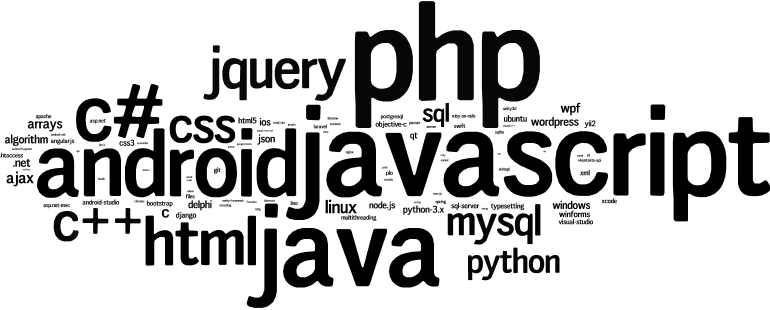
\includegraphics[width = 0.43\textwidth]{figures/toptagRSO.png}
		\label{fig:RSOtag}}
	\caption{Tag Cloud of Top Frequency Tags on ESO and RSO}
	\label{fig:tagclouds}
\end{figure}

However, we can also see that \textcolor{red}{the frequency of a tag may differ between the two sites, for example,} \textbf{php}(\#4 on ESO, \#1 on RSO), \textbf{winforms}(\#69 on ESO, \#29 on RSO), \textbf{ruby-on-rails}(\#15 on ESO, \#60 on RSO), etc.
Furthermore, 44 tags, such as \textbf{web-application}, \textbf{yii2}, \textbf{Unity3D}, etc., that appear in the top-100 list of Russian Stack Overflow also exist in English Stack Overflow, but they do not appear in the top-100 list of English Stack Overflow.
Similarly, 44 tags, such as \textbf{codeigniter}, \textbf{perl}, \textbf{maven}, etc.,that appear in the top-100 list of English Stack Overflow also exist in Russian Stack Overflow, but they do not appear in the top-100 list of Russian Stack Overflow.

To further understand the interest differences between the two sites, \textcolor{red}{we perform a Spearman Rank Correlation analysis of the ranks of the 2560 tags that are common in the two sites. 
Our results show that ... analyze the ranking correlation results ...
This suggests that although users of the two sites share much common interest in computer programming techniques, their level of interests in these techniques are different.}

%56 of the top-100 most frequently used tags in Russian Stack Overflow are also the top-100 most frequently
%And \textcolor{red}{56 CCY: we should tell the number of top-100 tags in RSO which are also covered in the whole SO.}of the top 100 frequent tags of Russian Stack Overflow also exist in the set of the top 100 frequent tags of Stack Overflow main site. 
%\textcolor{red}{CCY: We need a tag cloud for both RSO and SO to show the overlap between them.}
%As seen in Fig~\ref{fig:??}, most popular tags in the two sites are very similar which show the commonness between two sites.
%\textcolor{red}{CCY: Go on to add some other tags which appear much more frequently in Russian than that in overall Stack Overflow.}

\noindent \fbox{\centering%
	\parbox{1.0\textwidth}{%
		\textcolor{red}{will fix later ...}
		
		\textbf{Summary}:
		According to the tag analysis, majority of tags in Russian Stack Overflow are also on the main site. Moreover, it finds that Russian site is highly overlapped with the main site on the popular tags which indicate two sites may have very similar content among the popular topics. On the other hand, Russian site also has its unique tags whose related posts make an non-ignorable part of all posts. 


	}%
}
\\

\begin{comment}
	%Ranking the top 10 frequent tags in several sets to show what are the most popular fields in both sites.
\begin{table}[!h]
	\scriptsize
	\centering
	\caption{Top 10 Popular Tags Ranking Statics \textcolor{red}{1) How is freq \% calculated? Need to explain in the discussion. 2) Tags only in Russian should be a separate table. They are not top-10 popular tags.}}
	\label{tab:table4}
	\begin{tabular}{|p{0.8cm}<{\centering}|p{0.55cm}<{\centering}|p{0.8cm}<{\centering}|p{0.55cm}<{\centering}|p{1.5cm}<{\centering}|p{0.55cm}<{\centering}|}
	\hline
	{\scriptsize Main site tags} & freq. (\%) &{\scriptsize Russian site tags} & freq. (\%) &{\scriptsize Tags only in Russian site} & freq. (\%) \\
	\hline
	javascript & 3.39 & php & 6.51  & bootstrap  & 0.304 \\
	\hline
	java & 3.04 & javascript& 5.83  &\bf vkontakte-api & 0.200 \\
	\hline
	c\# & 2.63 & java & 5.31 & android-sdk & 0.178 \\
	\hline
	php & 2.59 & android & 4.43 & android-fragment & 0.143 \\
	\hline    
	android & 2.38 & c\#& 3.89 & mvc & 0.139 \\
	\hline    
	jquery & 2.01 & html & 3.21 & google-maps-api &0.109 \\
	\hline    
	python & 1.87 & jquery& 2.82 & golang & 0.106 \\
	\hline    
	html & 1.59 & c++ & 2.75 & cookie & 0.105 \\
	\hline    
	c++ & 1.23 & css & 2.47  & cms & 0.102 \\
	\hline    
	ios & 1.22 & mysql & 2.08  & \bf yandex-maps-api & 0.092 \\
	\hline 
	\end{tabular}
\end{table}		
\end{comment}

\begin{comment}
\begin{table}[!h]
	\scriptsize
	\centering
	\caption{Different tags preference between two sites \textcolor{red}{why this set of tags as examples? Please tell how do you get this set of tags.} \textcolor{blue}{XINGZC: In addition to showing some examples, I think we need to perform some statistical analysis of the ranks of all 2560 common tags in the two sites, which can show that whether the level of interests in these techniques are statically the same or different.}}
	\label{tab:table_tagpref}
	\begin{tabular}{|l l l l l|}
		\hline
		{\scriptsize Tags} & freq. in SO (\%) & freq. in RSO (\%) & Rank in SO & Rank in RSO \\
		\hline
		web-application & 0.047 & 0.49 & 322  & 32 \\
		\hline
		yii2 & 0.03 & 0.45 & 518  & 35 \\
		\hline
		cuda & 0.029 & 0.012 & 528 & 870 \\
		\hline
		winforms & 0.2 & 0.5 & 63 & 29 \\
		\hline    
		Unity3D & 0.08 & 0.029 & 175 & 58 \\
		\hline    
		website & 0.02 & 0.485 & 734 & 31 \\
		\hline    
		layout & 0.057 & 0.42 & 287 & 41 \\
		\hline    
		Joomla & 0.037 & 0.125 & 424 & 145 \\
		\hline    
	\end{tabular}
\end{table}	
\end{comment}

%According to the result shown in Table~\ref{tab:table4}, it is clear that the most popular areas of two sites are very similar. Though there is some difference among the \textcolor{red}{frequency numbers of the same tag ??you mean absolute frequency number? they are not comparable as the two site are of very different scale, not just due to different preference?} due to the different preference of two sites' users. Overall, 8 of the top 10 most popular tags on Russian site are also the top 10 popular tags on the main site. This indicates that the popular area and content between two sites are highly overlapped. However, focusing on some unique tags in Russian site, it appears some tags who also own considerable frequency. For example, {\bf Yandx}, which is {\bf \foreignlanguage{russian}{Яндекс} }in Russian, is a Russian multinational technology company specializing in search engine and it is the most used search engine in Russia.{\bf []} And {\bf VKontakte}, another Russian local company, is the biggest social network company in Russia and its website, vk.com, is the most popular webstie in Russia.{\bf []} It shows that the Russian sub-site does have some specialness in the content area.


\section{Knowledge Fragmentation and Duplication?: Evidences of Cross-Site Linking}
\textcolor{blue}{XINGZC: I did not revise this section as it does not seem ready for revision.}
Hyperlink is a good tool to recommend and refer the existing content to other users. 
%Not only links can refer the knowledge base in the same site, but also across different sub-sites, or external resources. 
%Under the site announcement of Japanese Stack Overflow, one user commented, ``''
As Stack Overflow and Russian Stack Overflow are both programming-related website, it is expected that some new questions asked in the Russian Stack Overflow may have already answered or highly related to Stack Overflow.
So there should be some mutual links between them.
In this section, we try to validate such assumptions with the analysis of existing links between them.
%In this section, we explore the relationships between Stack Overflow and Russian Stack Overflow according to their mutual hyperlinks. 
%The link amount and the direction reveal the similarity and difference between these two sites.

\noindent \fbox{\centering%
    \parbox{1.0\textwidth}{%
        \textit{``This is the world wide web and it is built on a thing called hypertext. Multiple languages? Cool, that's the "world" part. But don't forget about hypertext. Please, make sure that questions and answers can be linked easily across the different language sites. If someone asks a question in Japanese that is essentially a duplicate of an existing English question, linking the two questions will allow Japanese speakers (who might understand *some* English, or at least be able to read code snippets) to get immediate value from past answers, without waiting for new answers... ''
        }
        
        {\raggedleft --- one comment under the announcement of Japanese Stack Overflow\par}
            }%
}
\\

\begin{table}
	\caption{Links Statics}
	\centering
	\small
	\label{tab:links}
	\begin{tabular}{llll}
       \hline
		Source       &\#Total links & \#Links to SO   & \#Links to RSO\\ \hline
		SO Posts     & 13,636,973    & 1,581,888 (11.6\%)      & 88 \\
		SO Comments  & 5,959,110     & 1,835,405 (30.8\%)    & 164\\
		RSO Posts    & 131,964       & 5,674  (4.3\%)        & 5,014 (3.8\%) \\
		RSO Comments & 55,471        & 4,548  (8.2\%)        & 5,658 (10.2\%) \\
       \hline
	\end{tabular}

\end{table}	

\subsection{Explicit Cross-Site Links by Users}

In (Russian) Stack Overflow, users are allowed to add links in their posts (both questions and answers) and comments to refer to other resources. 
We count all links in two sites and analyse the link direction within and across two sites.
The statistics of links of two sites are summarised in Table~\ref{tab:links}.
Rarely, the links in Stack Overflow direct to Russian Stack Overflow.
But in contrast, many links in Russian Stack Overflow has been referring to Stack Overflow.
For example, in Russian Stack Overflow, 4.3\% links in posts and 8.2\% links in comments are referring to Stack Overflow.
However, compared with Russian Stack Overflow, we can see that 11.6\% links in posts and 30.8\% links in comments are from itself in Stack Overflow.
\textcolor{red}{CCY: this argument is a little far-fectched, how to say that more naturally in the paper?}
Such a large difference of link source leads to two potential reasons: 1) There is not enough overlap content between two sites; 2) Stack Overflow may be under-referenced in Russian Stack Overflow.
But as both Stack Overflow and the Russian one own millions of questions and answers, it is difficult for us to observe to determine which reason accounts for the relative small proportion of links to Stack Overflow.
Therefore, we propose a cross-site retrieval method to assist our observation and validate the reason mentioned above.
 
\begin{comment} 
Although the number seems not very big, but it is even more than the in-site links (3.8\%).
Furthermore, the links (8.2\%) in Russian Stack Overflow post to Stack Overflow is also comparable to itself (10.2\%).
Considering the links can be referring to any site in the world, this percentage is rather high, and it indicates the significant influence of Stack Overflow to the Russian one.
According to our observation, we find that the reason is like the posts in Figure~\ref{fig:answerExample}.
Some questions asked in Russian Stack Overflow are already asked or even answered in the main site, and the only difference is that it is expressed in Russian instead of English.	

But apart from existing mutual links between two sites, we find that some posts in Russian Stack Overflow are also highly related to posts in Stack Overflow, and such relationship has not been explicitly annotated by links.
For example, Fig~\ref{fig:??} shows two questions in two site respectively, and they express the same meaning, but the link to this earlier Stack Oveflow post does not appear in the later Russian post.\textcolor{red}{CCY: please find an example pair that one question in Stack Overflow is almost the same to one question in Stack Overflow, but such link has not been annotated.}
We conclude two reasons for the miss of such links.
First, the language gap between two sites limit the users in Russian Stack Overflow to find related English question.
Second, as Stack Overflow is larger and larger (tens of millions of questions and answers), it is difficult for users, especially non-native speakers to spot related questions in such a big corpus.
Therefore, a tool for finding related posts in two sites is highly needed to help bridge the gap between two sites, and also save time by avoiding duplicate efforts.
\end{comment}

\subsection{Implicit Cross-Site Links that Users Are Not Aware Of}

\begin{figure}
	\centering
	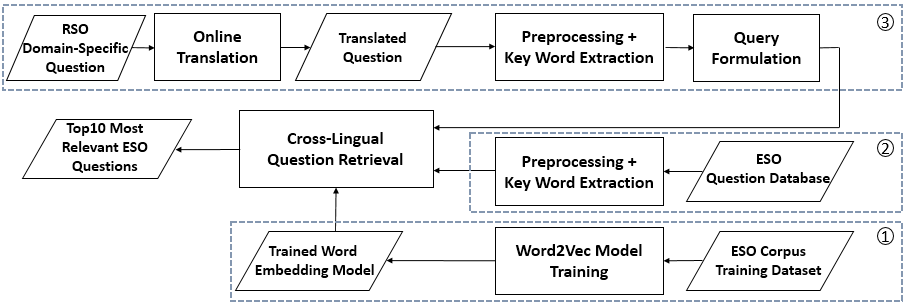
\includegraphics[width = 0.9\textwidth]{figures/workflow.png}
	\caption{Overall Framework for Cross-site Retrieval \textcolor{red}{CCY: 1) Do not need the ``Model Output Question''. 2) For English question, it also needs the ``key word extraction''. and put both the ``preprocessing'' and ``Key Word Extraction'' into a block with dilated box annotated as Step 5.}}
	\centering
	\label{fig:flowChart}
\end{figure}

\subsubsection{Method for cross-site retrieval}
Fig~\ref{fig:flowChart} displays the overall method to retrieve related questions in Stack Overflow.
The overall method can be separated into two parts i.e., prepare the posts from  ESO as the database, and then formulate the RSO questions as queries to retrieve related ESO questions.
Each question contains two parts, title and descriptions.
\begin{enumerate}
 \item Given one question in Russian Stack overflow, we first translate its title and content description into English with Google Translate\footnote{\url{https://cloud.google.com/translate}}.
 \item Then we preprocess the translated question by tokenzing the sentence, removing the stop words in both question's title and description.
 \item Then we extract the key words from the description part since there are irrelevant words in this part which could influence the model performance negatively. 
     To achieve this, we use two different popular keywords extraction algorithms (TF-IDF and TextRank\footnote{\url{https://github.com/davidadamojr/TextRank}}) to extract keywoords from the ESO question corpus. These two algorithms yield two different but 		     complementary sets of key words based on the offered corpus. To reduce the bias of using a single algorithm, we choose the union of the two keyword sets to build our final keywords extraction       	     vocabulary.
     Then we only select the keywords which appear in the vocabulary among the query description to improve the retrieval accuracy and speed.
 \item Next, we assign different weight to the keywords in title and description. As title represents more compact and meaningful information, we assign double weight to title words than description words.
 \item Then we also carry out the same preprocessing and keyword extraction to the ESO questions, and prepare them as the database for retrieval.
 \item To build the retrieval model, we adopt the word embedding model. Word embedding~\cite{??} is method to convert the words into dense vectors based on the assumption that words appear in similar context tend to have similar meanings. We trained an word embedding model on posts of Stack Overflow, and some examples can be seen in Fig~\ref{fig:wordEmbedding}. \textcolor{red}{Add a picture about word2vec + PCA} We can see that similar words \textcolor{red}{....} are relatively close in the vector space. Compared with traditional keyword match, word embedding model can help bridge the lexical gap between different words which share similar meanings. To calculate the relevance between the Russian query ($R$) and an English question ($E$) from the database, we first define the semantic similarity between a query word ($R_i$) and a question word ($E_j$) as the cosine similarity between their learned word embeddings, i.e., $Rel(R_i, E_j)=CosineSim(v_{R_i}, E_j)$. For each query word $R_i$, we compute its similarity with each word in the English Question and find the one with the largest similarity: 
 	 \begin{equation}
       Rel(R_i,E)=\max\limits_{j \in E}Rel(R_i, E_j)\times R_i.Weight
     \end{equation}

     We then define the relevance between a given query \emph{R} and an English question from database \emph{E} as 
      \begin{equation}
      	 \label{equ:relevance}
         Rel(R, E) = \sum_{j\in R}Rel(R_j, E)
      \end{equation}
     We will compare the query with all questions in our database, and sort the relevance value calculated by Equ.\ref{equ:relevance}.
     10 questions with the highest value are extracted as the most relevant questions.
 \end{enumerate}
 
\begin{comment}
%To ensure the translation quality, we also use a domain-specific vocabulary derived from the corpus of Russian Stack Overflow to translate the domain specific words, such as function, python and so on. 
Next, we assign the preprocessed title and preprocessed description key words to form the input query for the retrieval model (step4). 
we give the words in title and words in description different weight in the model caculation i.e., WT(word in title):WD(key word in description)=2:1. Before going into the model, prepared Stack Overflow database also go trough the same preprocessing as step2 to stay consistency with input query. 
To build the retrieval model, we use the pre-trained Word2Vec ~\cite{??} model to achieve word embedding on the input query and questions from Stack Overflow database. 
We use the entire corpus of collected English Stack Overflow database as the training data to make sure that most of the words appeared in our dataset  can be vectorized successfully. 
To caculate the relevance between the input query (\emph{q}) and an English question (\emph{Q}) from the database, we first define the semantic similarity between a query word (\emph{qw}) and a question word (\emph{Qw}) as the cosine similarity between their learned word embeddings, i.e., \emph{Rel(qw,Qw)=CosineSim(v$_{qw}$,v$_{Qw}$)}. 
After that, we use the text-to-text similarity measure introduced by Mihalcea et aI. ~\cite{??}. 
This measure defines the relevance between a query word (\emph{qw}) and a English question (\emph{Q}) is computed as the maximum similarity between (\emph{qw}) and any word \emph{w$^{'}$} in \emph{Q}, i.e., 

\begin{equation}
Rel(qw,Q)=\max\limits_{w^{'}\in Q}Rel(w^{'},qw)\times qw.Weight
\end{equation}

Finally, we define the relevance between a given query \emph{q} and an English question from database \emph{Q} as 

\begin{equation}
Rel(q,Q) = \sum_{qw\in q}Rel(qw,Q)
\end{equation}

According to the relevance value caculated through the above model, we can find the most 10 relevant questions related to the given russian question from the Stack Overflow database.
 
	
\end{comment}


\begin{figure}
	\centering
	\subfigure[\#44930249: No good solution on Russian Stack Overflow. \textcolor{red}{Show the answer to this English question} \textcolor{blue}{You can read first 2 sentences carefully, actually this user's English is poor.}]{
		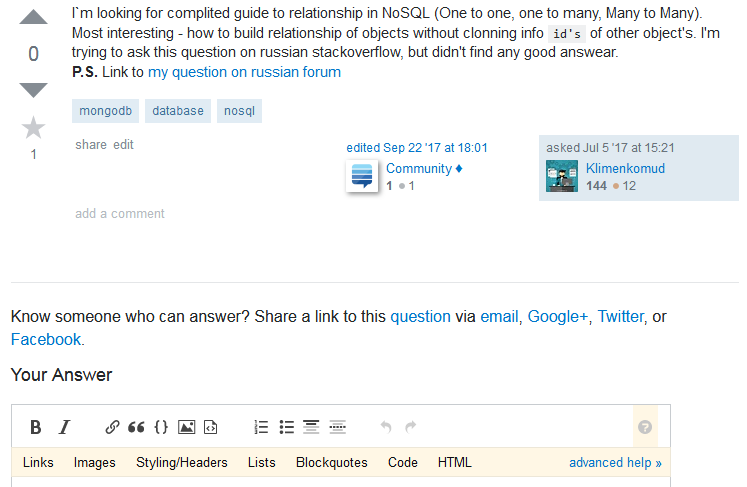
\includegraphics[width = 0.43\textwidth]{figures/introex1.png}
		\label{fig:SOquestionExample}
	}
	\hfill
	\subfigure[\#479080: Exist good solutions on the Stack Overflow. \textcolor{red}{This is an answer, right? Show the Russian question of this answer. Show the referenced Stack Overflow main site post}]{  
		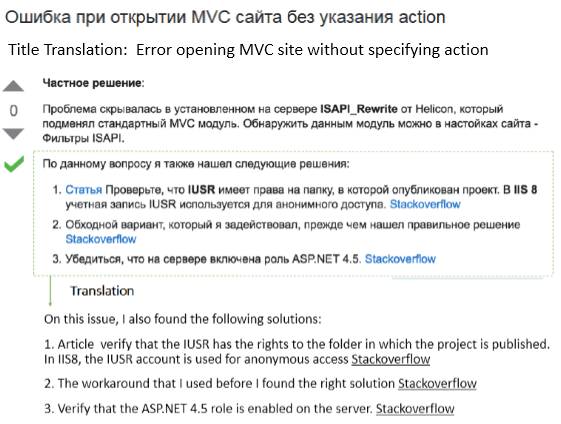
\includegraphics[width = 0.43\textwidth]{figures/introex2.png}
		\label{fig:RSOanswerExample}
	}
	\caption{Some cases found on Stack Overflow sites \textcolor{red}{I understand you use these two examples to illustrate the need for cross-reference between main site and lingual-variant. But will they incur questions? Because they show that main site and lingual-variant users can cross-reference posts on the two sites. For (a), ``This user can ask question very well in English. So he does not really need our tool support''. For (b), ``This user can well reference main site posts in their answers. So no need for our tool support either''. I think we also need another example ``A Russian question no body answers. No cross-reference to main site post. but there is actually a very relevant main site post that can answer the no-body-answer Russian question''. This example will show that there are implicit cross-site knowledge to discover and utilize, in addition to those manual-cross-site references.} \textcolor{blue}{CCY:Actually, I want to use these examples to show the relationships between two sites. I think that it is not necessary to show the need of the cross-reference in the introduction as it is too sudden and early for readers to understand. So I put the need of more cross-site reference into Section 2.2.3.}\textcolor{red}{QZQ: will add the two new examples later}}
	\label{fig:linkPair}
\end{figure}


\subsubsection{Manual validation of cross-site reference}
In Russian Stack Overflow, one question may contain a link to posts (question or answer) in Stack Overflow.
We assume that such a link represents that the source question in Russian Stack Overflow is identical to the target question in Stack Overflow.
Our task is to see if that assumption holds by checking the retrieval result of our searching model mentioned above.
We totally collect 5,035 link pairs.
As we are most familiar with \textit{Python} related questions, we randomly select 50 link pairs whose both source question in Russian Stack Overflow and target question in Stack Overflow are attached with tag \textit{Python}.
There are totally 779,370 questions chosen from Stack Overflow as the candidate for the query.
Then we take the question (title and description) in Russian Stack Overflow as the query, and our model returns top-10 related questions in Stack Overflow.
The results show that 29 (58\%) of the ground truth are in the top-10 recommendations.
Then we manually check why the other 21 queries cannot get satisfying results, and conclude two main reasons.
First, some reference link are not right or not most suitable ones.
\textcolor{red}{QZQ:new examples.} 
For instance, there is a Russian question, \foreignlanguage{russian}{"Почему нет исключения TypeError?"}\footnote{\url{https://ru.stackoverflow.com/questions/564442/}}, which can be translated as "Why is there no TypeError exception?".
On the other hand, there is a link in this question leading to the question English on Stack Overflow whose title is "In Python, how do I determine if an object is iterable?"\footnote{\url{https://stackoverflow.com/questions/1952464/}}. 
After manually checking this one pair on the Stack Overflow, it is easy to find the russsian question is asking about how to solve a type error in its code. Whithin the question description, the question's owner mentioned one possiblity causing the error and refered the link to explain his assumption. So this refered English question is talking about another topic which actually can not deal with this error. So this reference link is not the most suitable one to descripe or solve this russian question.

Here is another example, one Russian question's title is \foreignlanguage{russian}{"Почему не работает унаследованная форма?"}\footnote{\url{https://ru.stackoverflow.com/questions/318618/}}, which is translated as "Why does not the inherited form work?". 
It has a link to an English question on Stack Overflow, "why does not work in the form of validation?"\footnote{\url{https://stackoverflow.com/questions/23534615}}. 
After checking these two question, we find that the Russian question owner want to find a solution to solve his problem but he mentioned that the method in the refered English question was not working. So the reference here is a counter-example. 

Second, the reference which can not be spotted by our method is due to the limitation of our model. 
Our model focus on capturing and computing the semantic difference between the input words, so currently it may not work well with some deep semantic relationship between words. 
For instance, given an RSO question "\foreignlanguage{russian}{Порядок удаления элементов списка в python}"\footnote{\url{https://ru.stackoverflow.com/questions/55464/}} (translated as "the removal of elements of the list in python"), 
the link inside leads to an English question, "Calling 'del' on a list"\footnote{\url{https://stackoverflow.com/questions/8205102/}}.
In this example, 'del' is obviously a function name for deleting.
However, currently, our model is not able to capture such domain-specific information.
%For human, we can easily find the strong relationship between 'del' function and 'removal of elements' but such a deep relationship cannot be captured by our current Word2Vec model. 
%Another example is a russain question, whose title is \foreignlanguage{russian}{Почему нет исключения TypeError?}, translated as \emph{why there is no exception TypeError?} . The question owner post a link to Stack Overflow, whose pointed question is with the title, \emph{ In Python, how do I determine if an object is iterable?}. After we check these two question on both site, we do find they are highly related. But these two question are too different semanticaly by using many different words to descripe similar situation. So this kind of special case cannot be handled well by our current model.

 We then take the other 50 \textit{Python} questions randomly from Russian Stack Overflow which do not contain any links to Stack Overflow.
 We regard them as the queries, and to see if we can find any identical questions in Stack Overflow.
 We manually check the results and find that for \textcolor{red}{23 (46\%)} of them, we can locate similar questions in top-10 relevant results from our model. 
Here are three examples\footnote{\url{https://ru.stackoverflow.com/questions/464/}}\footnote{\url{https://ru.stackoverflow.com/questions/432934/}}\footnote{\url{https://ru.stackoverflow.com/questions/420125/}} in table~\ref{tab:reviewresult} from the experiment result. 
To save space, we only update the top 3 most relevent questions yielded by our model. 
 \textcolor{red}{Find an example of }
 \textcolor{red}{.....}

 \begin{table}
 \caption{Examples from no-link related validation experiment \textcolor{red}{1) For the first column, do follow my ASE'16 paper to draw the figure or Qiancheng's 4.0 version.QZQ:will improve the layout later. example 2 and 3 are new}}
 \centering
 \tiny
 \label{tab:reviewresult}
 \begin{tabular}{|p{1cm}|p{4cm}|p{4cm}|p{4cm}|}
 	%\hline
	%Russian Question &{\emph \foreignlanguage{russian}{IDE для Python}} & {\emph \foreignlanguage{russian}Отладка кода на Питоне}} &{\emph \foreignlanguage{russian} {Python обработчик системного меню Windows}\\ 
 	\hline
 	Translated Question & IDE for python & the slow implement of the code, a coin toss & books and educational resources for python\\
 	\hline
 	Result \#1 & Searching for a Python lightweight IDE (or text-editor) & python code for coin toss issues & Resource/book suggestion to effectively writing software for python/c++ beginer\\
 	\hline
 	Result \#2 & What's a good IDE for Python on Mac OS X? & python coin toss & good resource for learning advanced or obscure python concepts \\
 	\hline
 	Result \#3 & IDE for Python: test a script & Simulate multipe coin toss streak & what are good online resources to learn using Pyhton to get and post data in a webpage?\\
	
 	\hline
 \end{tabular}
 
 \end{table}


\textbf{Summary}: 
Many hyperlinks in Russian Stack Overflow come from the main site which shows the Stack Overflow is an important information resource for the Russian one.
But there are still two problems with it, one is that some existing links are not related or not most related.
Second, some reference links are missing and need the support of some tools.
